%%%%%%%%%%%%%%%%%%%%%%%%%%%%%%%%%%%%%%%%%
% Beamer Presentation
% LaTeX Template
% Version 1.0 (10/11/12)
%
% This template has been downloaded from:
% http://www.LaTeXTemplates.com
%
% License:
% CC BY-NC-SA 3.0 (http://creativecommons.org/licenses/by-nc-sa/3.0/)
%
%%%%%%%%%%%%%%%%%%%%%%%%%%%%%%%%%%%%%%%%%

%----------------------------------------------------------------------------------------
%	PACKAGES AND THEMES
%----------------------------------------------------------------------------------------

\documentclass{beamer}
%\usepackage{extrabeamercmds}

\usepackage{amsmath}
\usepackage{movie15}
\usepackage{hyperref}
\usepackage{float}
\usepackage{amsmath}
\usepackage{ amssymb }
%\usepackage[caption = false]{subfig}
\bibliographystyle{abbrv}
\usepackage{graphicx}
\usepackage{caption}
\usepackage{subcaption}
\usepackage{tikz}
\usetikzlibrary{shapes,arrows,positioning}

\setbeamertemplate{blocks}[rounded][shadow=false]

%A few commonly used constants, to cut down on typing and increase clarity
\def\eps0{\ensuremath{\epsilon _0}}
\def\2pieps0{\ensuremath{2\pi \epsilon _0}}
\def\4pieps0{\ensuremath{4\pi \epsilon _0}}
\def\k{\ensuremath{\displaystyle \frac{1}{4\pi \epsilon _0}}}
\def\muz{\ensuremath{\mu_0}} %For some reason, \mu0 gave me an error - probably because \mu is a command

%Define a closed integral construct. I had some help with making this one look nice
\def\cint#1{\ensuremath{\displaystyle\underset{\substack{\text{\tiny{closed}}\\\text{\tiny{surface}}}}{\oint} \mspace{-0.1 mu} #1}}

%Define symbols for flux, just to make sure it stays consistent throughtout the paper
\def\phie{\ensuremath{\phi_E}}
\def\phib{\ensuremath{\phi_B}}

%Define the derivatives I'll be using, so I don't have to do all the typing every time
\def\dA{\ensuremath{\emph{d}\vec{A}}}
\def\dB{\ensuremath{\emph{d}\vec{B}}}
\def\ds{\ensuremath{\emph{d}\vec{s}}}
\def\dt{\ensuremath{\emph{dt}}}
\def\dphie{\ensuremath{\emph{d}\phie}}
\def\dphib{\ensuremath{\emph{d}\phib}}

% dx in the integral equations
\newcommand*\diff{\mathop{}\!\mathrm{d}}
\newcommand*\Diff[1]{\mathop{}\!\mathrm{d^#1}}
\tikzset{block/.style={rectangle, draw, fill=blue!20, text width=5em, text centered, rounded corners,
 minimum width=3.5cm}}
\tikzset{line/.style={draw, -latex}}
\beamertemplatenavigationsymbolsempty

\mode<presentation> {

% The Beamer class comes with a number of default slide themes
% which change the colors and layouts of slides. Below this is a list
% of all the themes, uncomment each in turn to see what they look like.

%\usetheme{default}
%\usetheme{AnnArbor}
%\usetheme{Antibes}
%\usetheme{Bergen}
%\usetheme{Berkeley}
%\usetheme{Berlin}
%\usetheme{Boadilla}
%\usetheme{CambridgeUS}
%\usetheme{Copenhagen}
%\usetheme{Darmstadt}
%\usetheme{Dresden}
%\usetheme{Frankfurt}
%\usetheme{Goettingen}
%\usetheme{Hannover}
%\usetheme{Ilmenau}
%\usetheme{JuanLesPins}
%\usetheme{Luebeck}
\usetheme{Madrid}
%\usetheme{Malmoe}
%\usetheme{Marburg}
%\usetheme{Montpellier}
%\usetheme{PaloAlto}
%\usetheme{Pittsburgh}
%\usetheme{Rochester}
%\usetheme{Singapore}
%\usetheme{Szeged}
%\usetheme{Warsaw}

% As well as themes, the Beamer class has a number of color themes
% for any slide theme. Uncomment each of these in turn to see how it
% changes the colors of your current slide theme.

%\usecolortheme{albatross}
%\usecolortheme{beaver}
%\usecolortheme{beetle}
%\usecolortheme{crane}
%\usecolortheme{dolphin}
%\usecolortheme{dove}
%\usecolortheme{fly}
%\usecolortheme{lily}
%\usecolortheme{orchid}
%\usecolortheme{rose}
%\usecolortheme{seagull}
%\usecolortheme{seahorse}
%\usecolortheme{whale}
%\usecolortheme{wolverine}

%\setbeamertemplate{footline} % To remove the footer line in all slides uncomment this line
%\setbeamertemplate{footline}[page number] % To replace the footer line in all slides with a simple slide count uncomment this line

%\setbeamertemplate{navigation symbols}{} % To remove the navigation symbols from the bottom of all slides uncomment this line
}

\usepackage{graphicx} % Allows including images
\usepackage{booktabs} % Allows the use of \toprule, \midrule and \bottomrule in tables

%----------------------------------------------------------------------------------------
%	TITLE PAGE
%----------------------------------------------------------------------------------------

\title[FreeSurfer]{Extraction of Mesh from FreeSurfer} % The short title appears at the bottom of every slide, the full title is only on the title page

\author{Lars Magnus Valnes} % Your name
\institute[UiO] % Your institution as it will appear on the bottom of every slide, may be shorthand to save space
{
University of Oslo \\ % Your institution for the title page
%\medskip
%\textit{john@.com} % Your email address
}
\date{\today} % Date, can be changed to a custom date

\begin{document}




%&&&&&&&&&&&&&&&&&&&&&&&&&&&&&&&&&&&&&&&&&&&&&&&&&&&&&&&&&&&&&&&&&&&&&&&&&&&&&&&&&&&&&&&&&&&&&&&&
\begin{frame}
\titlepage % Print the title page as the first slide
\end{frame}

%&&&&&&&&&&&&&&&&&&&&&&&&&&&&&&&&&&&&&&&&&&&&&&&&&&&&&&&&&&&&&&&&&&&&&&&&&&&&&&&&&&&&&&&&&&&&&&&&

%================================================================================
\section{Introduction}
%================================================================================


%---------------------------------------------------------------------------------------------------------------------------------------------
%	Slide 1a
%---------------------------------------------------------------------------------------------------------------------------------------------


%\begin{frame}{Introduction}
%\begin{block}{Goals}
%\begin{itemize}
%\item Basic understanding of Freesurfer 
%\end{itemize}
%\end{block}
%\end{frame}
%
%%---------------------------------------------------------------------------------------------------------------------------------------------
%%	Slide 1b
%%---------------------------------------------------------------------------------------------------------------------------------------------
%
%\begin{frame}{Introduction}
%\begin{block}{Goals}
%\begin{itemize}
%\item Basic understanding of Freesurfer
%\item Know how to extract a binary surface file from Freesurfer 
%\end{itemize}
%\end{block}
%\end{frame}
%
%%---------------------------------------------------------------------------------------------------------------------------------------------
%%	Slide 1c
%%---------------------------------------------------------------------------------------------------------------------------------------------
%
\begin{frame}{Introduction}
\begin{block}{Goals}
We some goals for today :
\begin{itemize}
\item<2-> Basic understanding of FreeSurfer 
\item<3-> Know how to extract a binary surface file from FreeSurfer. 
\item<4-> Construction of a mesh with mshr.
\end{itemize}
\end{block}
\end{frame}

%\begin{frame}{Freesurfer}
%\begin{block}{Cortical Parcellation}
%Cortical Parcellation ?? 
%\begin{itemize}
%\item<2-> ?
%\end{itemize}
%\end{block}
%\end{frame}



\section{FreeSurfer}
\begin{frame}{FreeSurfer}
\begin{block}{Introduction}
Some basic things about FreeSurfer.
\begin{itemize}
\item<2-> FreeSurfer is a set of software tools for the study of cortical and subcortical anatomy structures.
\item<3-> Most of FreeSurfer is automated. Thus simple to use, but not to debug.
\item<4-> The code written in C and based on ITK (National Library of Medicine Insight Segmentation and Registration Toolkit).
\end{itemize}
\end{block}
\end{frame}

\begin{frame}{FreeSurfer}
\begin{block}{Setting up FreeSurfer}
\begin{itemize}
\item<2-> Download from \href{http://freesurfer.net/fswiki/Download}{\beamergotobutton{here}} and obtain license.txt \href{https://surfer.nmr.mgh.harvard.edu/registration.html}{\beamergotobutton{here}}
\item<3-> FreeSurfer require that we set some environment variables.
\item<4-> This can be done by modifying .bashrc or .tcshrc.
\item<5-> Two useful environment variables to know are:
	\begin{itemize}
	\item<6-> \$FREESURFER\_HOME 
    \item<6-> \$SUBJECTS\_DIR 
	\end{itemize}
\end{itemize}
\end{block}
\end{frame}


\begin{frame}{FreeSurfer}
\begin{block}{Running FreeSurfer}
\visible<1->{
The first step is to input the MRIs to FreeSurfer, this is done by typing: }\\ 
\visible<2->{
\$recon-all -subjid NAME -i PATH2MRI}  \\
\visible<3->{
Here NAME refers to what you want the folder in \$SUBJECT\_DIR to be named, and it  will store all the output related to the MRI.} \\
\visible<4->{
PATH2MRI refers to the complete path to a nifti file or a single DICOM file in a serie.} \\
\visible<5->{
The next step is to type :} \\
\visible<6->{
\$recon-all -subjid NAME -all }\\
\visible<7->{
The flag -all will initialize a complete FreeSurfer process.}
  
\visible<8->{
The process is stepwise and each step is described  \href{https://surfer.nmr.mgh.harvard.edu/fswiki/recon-all}{\beamergotobutton{here}}.}\\
\visible<9->{
For more through details, I recommend reading the relate articles found 
\href{https://www.zotero.org/freesurfer/items/collectionKey/F5C8FNX8}{\beamergotobutton{here}}.}
\end{block}
\end{frame}

\begin{frame}{FreeSurfer}
\begin{block}{Output Structure in FreeSurfer}
The output will be written to folders in \$SUBJECTS\_DIR/subjid, and we can look at the folders by typing : \\
\pause
\$recon-all -subjid name -i path\_to\_dicom \\ 
\$ls \$SUBJECTS\_DIR/name\\ 
\end{block}
\end{frame}

\begin{frame}{FreeSurfer}
\begin{block}{File Formats in FreeSurfer}
FreeSurfer will generate many different types of files, thus we will have a short introduction to a selected few.
\begin{itemize}
\item<2-> The extension .mgh is volume of voxels and a compressed .mgh file has the the extension .mgz.
\item<3-> Surface files, which are 3D triangulated binary surface files. 
\item<4-> Label are text files with vertices and corresponding values ( integer or string), \href{run:./Files/lh.BA1.label}{\beamergotobutton{Label file}}
\item<5-> Annotation files contains a collection of labels, and also includes a colour table     
\item<6-> Atlas contains probabilistic information estimated to label neuroanatomy each location on a cortical surface model. 
\item<7-> Template used to analyse longitudinal volumes.

\end{itemize}
\end{block}
\end{frame}



\begin{frame}{FreeSurfer}
\begin{block}{Surface Files}
For this presentation we will focus on surface files, and there are different types : 
\begin{itemize}
\item<2-> ?h.pial surface displays gyri and sulci, the sulci is barely visible.
\item<3-> ?h.white surface displays boundary between white and grey matter.
\item<4-> ?h.inflated surface shows fully the sulci.   
\end{itemize}
\end{block}
\visible<5-> { 
\begin{figure}
\centering
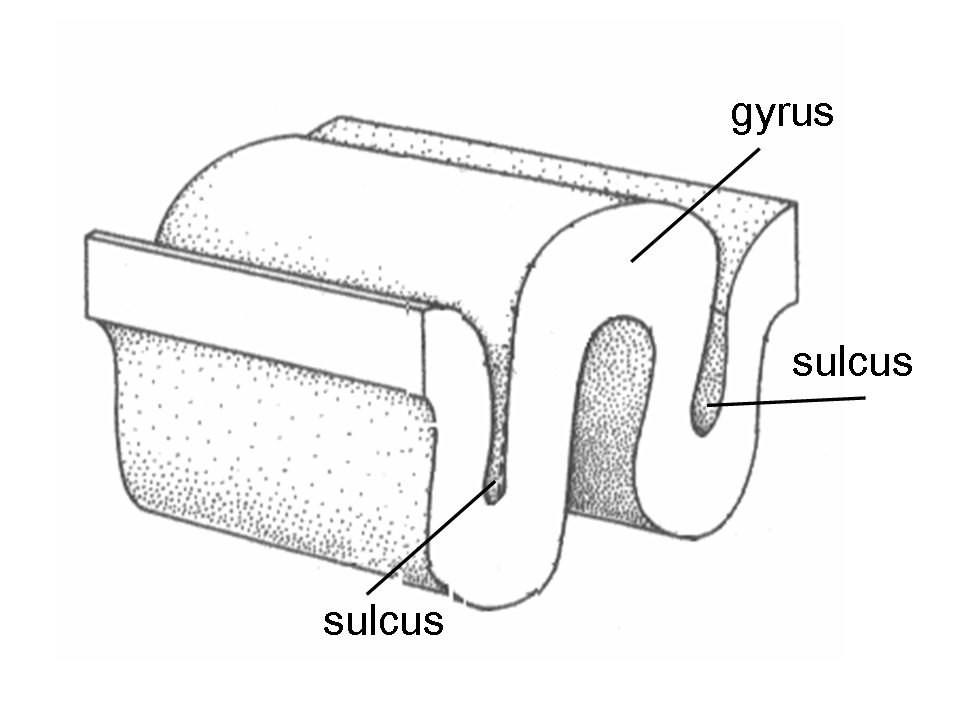
\includegraphics[scale=0.25]{Gyrus_sulcus.png} 
\end{figure}}

\end{frame}

\begin{frame}{FreeSurfer}
\begin{block}{Coordinate Systems}
FreeSurfer works with multiple coordinate systems, and we will look at most of them.
	\begin{itemize}
	\item<2-> Scanner-space, often LPS (Left Posterior Superior)     
	\item<3-> Voxel coordinates, (256,256,256) 
	\item<4-> Scanner RAS-coordinates, stands for Right Anterior Superior
	\item<5-> TkReg-RAS , the coordinate system for tksurfer and surfaces. 
\end{itemize}
\visible<6->{More details are found \href{run:./Files/fscoordinates.pdf}{\beamergotobutton{here}}.}
\end{block}
\end{frame}


\begin{frame}{FreeSurfer}
\begin{block}{Freeview}
Freeview is graphic user interface for FreeSurfer, and can be opened by typing :\\

\$ freeview.
\pause
\begin{itemize}
\item<3-> We can also add flags with more specifications:
	\begin{itemize}
	\item<4-> -v  \$SUBJECTS\_DIR/bert/mri/aseg.mgz:colormap=lut:opacity=0.2
	\item<4-> -f  \$SUBJECTS\_DIR/bert/surf/rh.white:edgecolor=blue 
	\item<4->  \small{-f  \$SUBJECTS\_DIR/bert/surf/lh.white:annot=aparc.annot:name=pial \_aparc:visible=0 }
	\end{itemize}
\end{itemize}
\end{block}
\end{frame}

\section{Freeview}
\begin{frame}{Freeview}
\begin{block}{Working in Freeview}
When working with surface files, it can be 
\begin{itemize}
\item<2-> Overlay, load a thickness file to see the thickness of the surface.   
\item<3-> Annotation, will display a collection of labels on a surface.
\item<4-> Curvature, shows the curvature of the surface.
\item<5-> Label, will highlight a specific part of the surface.
\end{itemize}
\end{block}
\end{frame}





\begin{frame}{Mesh Extraction}
\begin{block}{Introduction}
Mesh extraction is to obtain a 3D triangulated surface file from Freesurfer and we will look at :
	\begin{itemize}
	\item<2-> Scripts from brainder.org. % Give credit where credit is due
	\item<3-> FreeSurfer commands	
	\end{itemize}
\end{block}
\end{frame}

\begin{frame}{Mesh Extraction}
\begin{block}{Command for extraction of a 3D triangulated surface file.}
If we have a 3D triangulated surface file, we can simply type : \\ 
\small{
 \$mkdir \$SUBJECTS\_DIR/bert/asc    \\
\$mris\_convert \$SUBJECTS\_DIR/bert/surf/lh.pial  \\ \hspace{3cm} \$SUBJECTS\_DIR/bert/asc/lh\_pial.asc 
}
\end{block}
\end{frame}

\begin{frame}{Mesh Extraction}
\begin{block}{Brainder scripts}
Brainder.org is a sharing website with application towards FreeSurfer.
\begin{itemize}
\item<2-> Generating the surfaces for subcortical structures, aseg2srf.sh 
\item<3-> Importing FreeSurfer cortical meshes into Blender , srf2obj.gawk 
\end{itemize}
\end{block}
\end{frame}

\begin{frame}{Mesh Extraction}
\begin{block}{The Script aseg2srf.sh}
\begin{itemize}
\item<2-> Obtains the mesh from a volume of voxels. 
\item<3-> Can have topological defects.
\item<4->  \href{run:./Files/aseg2srf.sh}{\beamergotobutton{aseg2srf.sh}}
\end{itemize}
\end{block}
\end{frame}


%\begin{frame}{FreeSurfer}
%
%\begin{center}
%
%\scalebox{0.6}{
%      \begin{tikzpicture}[node distance=2.3cm]
%        \node  [block] (atlas){Atlas};
%        \node  [block,below of=atlas] (annotation){Annotation};
%        \node  [block,below of=annotation] (labels){Labels};
%        \path [line] (atlas) -- (annotation) ;
%        \path [line] (annotation) --(labels);
%      \end{tikzpicture}%
%}      
%\end{center}
%\end{frame}


\begin{frame}{Surface Generation}
\begin{block}{Commands for Skull Surface}
We can also obtain surfaces by adding optional inputs to FreeSurfer commands. \\
\small{
\qquad \$mri\_watershed -useSRAS -surf \\ \hspace{2.5cm} \$SUBJECT\_DIR/bert/surf/outer \\ \hspace{3cm} \$SUBJECT\_DIR/bert/mri/orig\_nu.mgz \\ \hspace{3.5cm} \$SUBJECT\_DIR/bert/trash/trash.mgz 
}
\\ \pause
This command will generate four surfaces : 
\begin{itemize}
\item<2-> Inner skull 
\item<3-> Outer skull
\item<4-> Outer skin
\item<5-> Brain surface
\end{itemize}
\end{block}
\end{frame}

\begin{frame}{Mesh Extraction}
\begin{block}{Inner and Outer Skull}
\begin{figure}
\centering
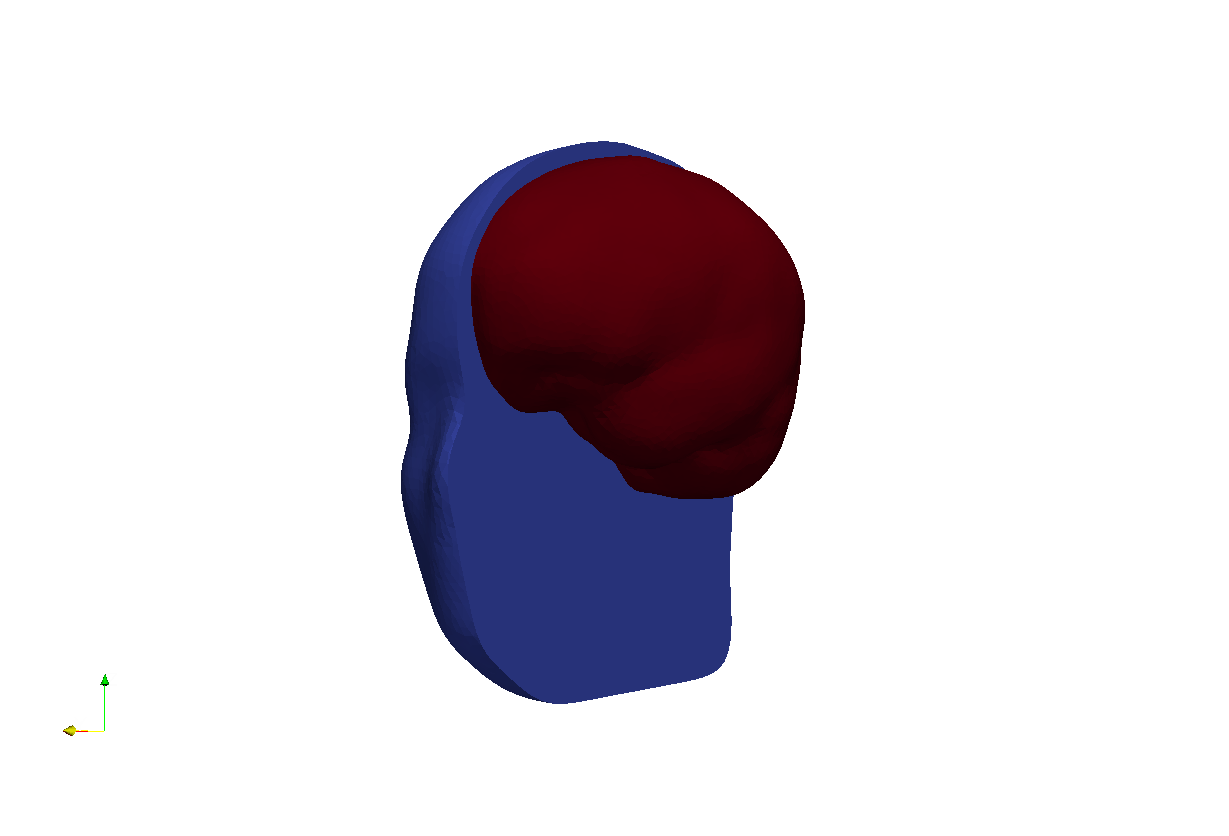
\includegraphics[scale=0.23]{skull.png} 
\end{figure}
\end{block}
\end{frame}





\section{Mesh Extraction}

\begin{frame}{Mesh Extraction}
\begin{block}{Surf2Mesh}
\begin{itemize}
\item<2-> A set of scripts to create a mesh from a .asc file can be seen  \href{https://github.com/larsmva/Surf2Mesh}{\beamergotobutton{here}}.
\item<3-> Contains .asc to .off/.stl conversion, will preferably become obsolete.
\item<4-> Also there are some scripts to simplify the mesh creation. 
\item<5->  \href{run:./Files/Extmesh_utility.py}{\beamergotobutton{Extmesh\_utility.py}}
\end{itemize}
\end{block}
\end{frame}

\begin{frame}{Mesh Extraction}
\begin{block}{Viewing Mesh in Paraview}
\begin{figure}
\centering
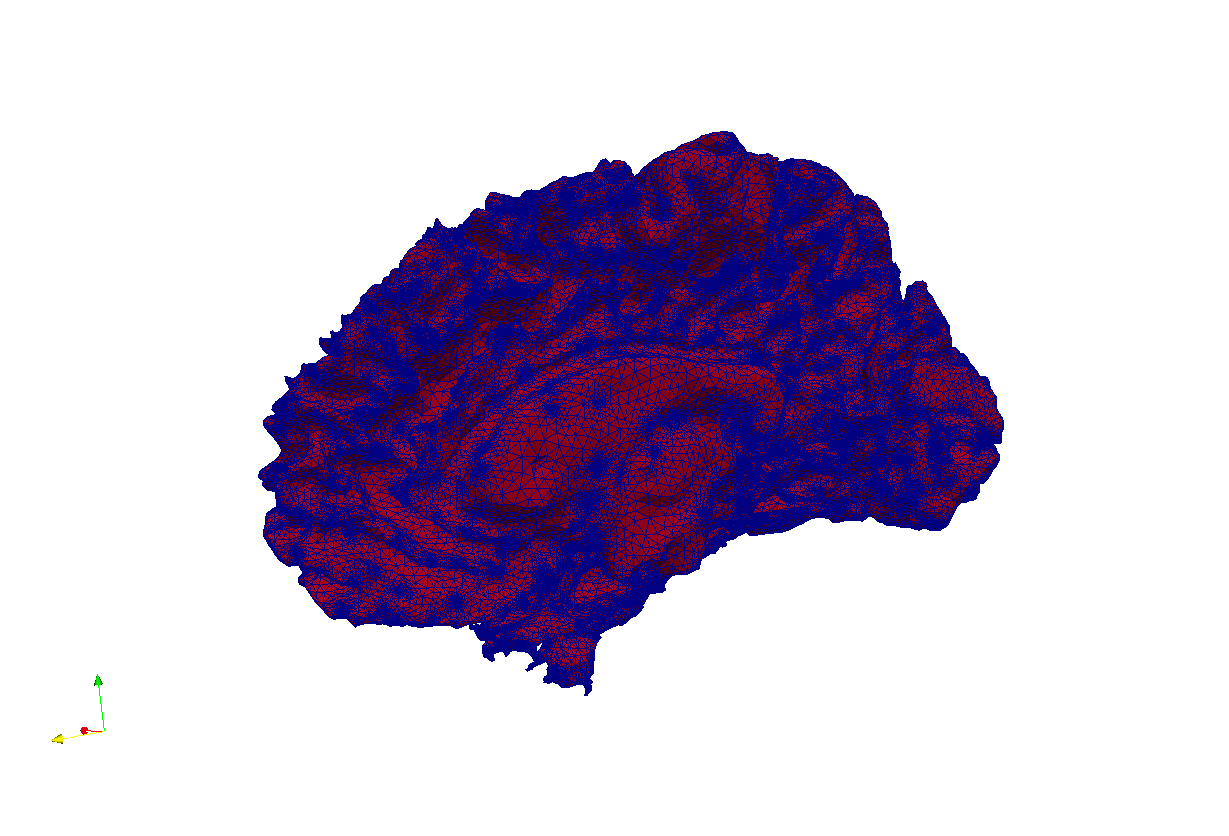
\includegraphics[scale=0.23]{white_mesh.png} 
\end{figure}
\end{block}
\end{frame}



\begin{frame}{Ending}
\begin{block}{Future}
\begin{itemize}
\item<2-> Python module Nibabel.
\item<3-> Register commands. 
\item<4-> Accurately marking subdomains of extracted mesh. 
\end{itemize}
\end{block}
\end{frame}


%\begin{frame}{Brainder}
%\begin{block}{Code}
%\begin{itemize}
%\item Brainder code is built using Freesurfer commands
%\item - mri_pretess , 
%\item - mri_tessellate ,
%\item - mris_smooth , used to smooth the surface
%\item - mris_convert ,
%\end{itemize}
%\end{block}
%\end{frame}

\end{document}
